
%opening
\title{Entwicklung des Layouts des Browsers}
\author{Burak Erol, Andreas Netsch, Philipp Winterholler}

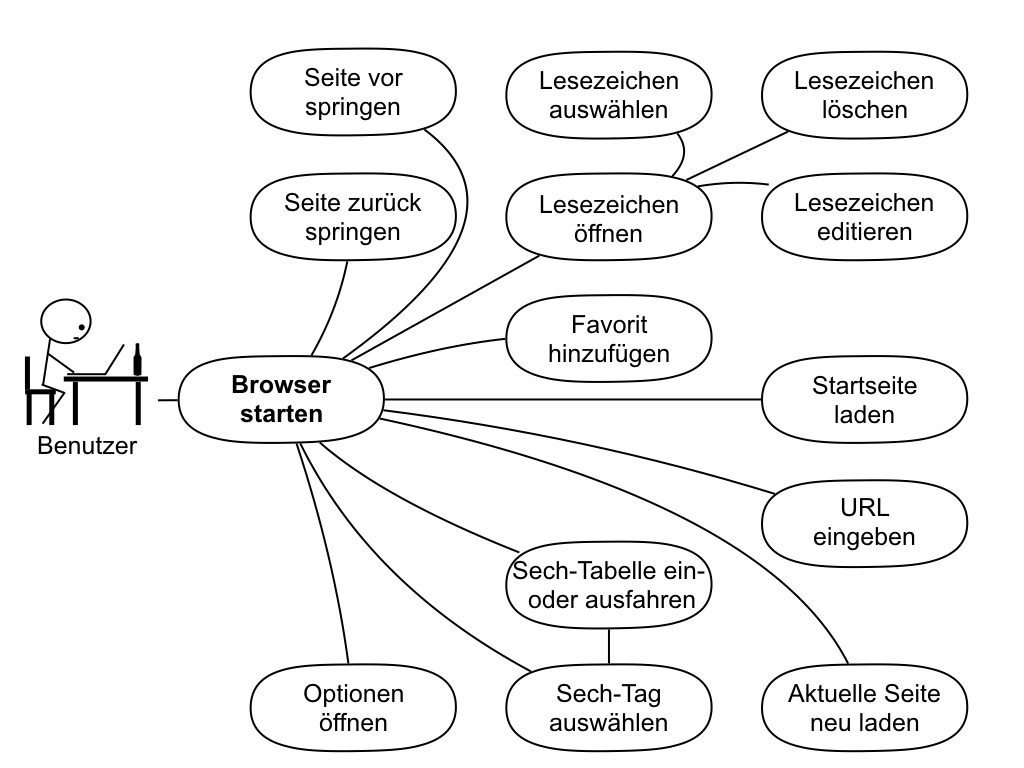
\includegraphics[width=12cm]{Pics/use_case_browser}

\section{Entwicklung des Layouts des Browsers}

Das Layout des Browsers besteht aus folgenden Elementen:

- Navigation Controller
- Navigation Bar
	- Back/Forward Button
	- Lesezeichen Button
	- Lesezeichen hinzuf��gen Button
	- Home Button
	- AddressBar
	- Reload Button
	- Sech Button
	- Optionen Button
- Container
- WKWebView

Die oben aufgelisteten Elemente stellen das komplette Layout des Browser dar. Der Navigation Controller dient in diesem dazu, dem Browser einen automatisch generierten Navigation Bar hinzuzuf��gen, welche im oberen Bildschirm fest verankert ist und eine nicht ver�nderbare H�he und Breite liefert. Diese Navigation Bar besitzt einen Back Button, um auf einer Seite zur�ck zu springen und einen Forward Button, um eine Seite vor zu bl�ttern. Bedient man den Lesezeichen Button so �ffnet sich eine TableView mit aller gespeicherten Seiten chronologisch absteigend in der er eine Seite ausw�hlen, l�schen oder editieren kann. Will der Nutzer die Liste um ein weiteres Element erg�nzen, so muss er den Plus Button bedienen und es �ffnet sich ein Pop Up Fenster, der den Link der aktuell besuchten Seite automatisch ��bernimmt und der Nutzer diesem jediglich nur noch einen Titel vergeben und abspeichern muss. Mit dem Home Button gelangt der Nutzer zu seiner definierten Startseite. Die AddressBar dient f��r die Eingabe eines Weblinks der durch best�tigen zu der eingegeben Seite gelangt. Um die aktuelle Seite neu zu laden, muss der Reload Button bedient werden. Will der Benutzer alle Sech Tags auf der aktuellen Seite anzeigen, so bedient er den Sech Button. Ist der Sech Button angeklickt worden, so klappt sich von der rechten Bildschirmseite eine TableView mit allen Sech Tags auf und bietet dem Nutzer eine �bersicht dieser. Wird eines der Sech Tags in dieser TableView angeklickt, so �ffnet sich ebenfalls ein PopUp Fenster zu diesem Tag, der weitere Informationen zur��ckliefert. Um die Sech Tag Tabelle wieder einzuklappen wird ein weiteres Klicken auf den Sech Button ben�tigt und diese f�hrt sich ein. Durch einen Klick auf den Optionen Button �ffnet sich auch hier ein Pop Up Fenster, der benutzerspezifische Informationen mitliefert und �bersichtlich darstellt. Um den WKWebView eine dynamische H�he und Breite programmatisch zu ��bergeben, wurde ein Container, eine Schicht unter diesem, mit festen Constraints �bergeben. Diese Constraints passen sich zu den benachbarten Elementen, wie der ausgefahrenen Sech Tabelle oder der Navigation Bar, an und das WKWebView �bernimmt die Constraints dieses darunter liegenden Containers. Dreht man das Endger�t beispielsweise von Hochformat in den Querformat, �ndern sich H�he und Breite des Containers und diese werden vom WKWebView �bernommen. 

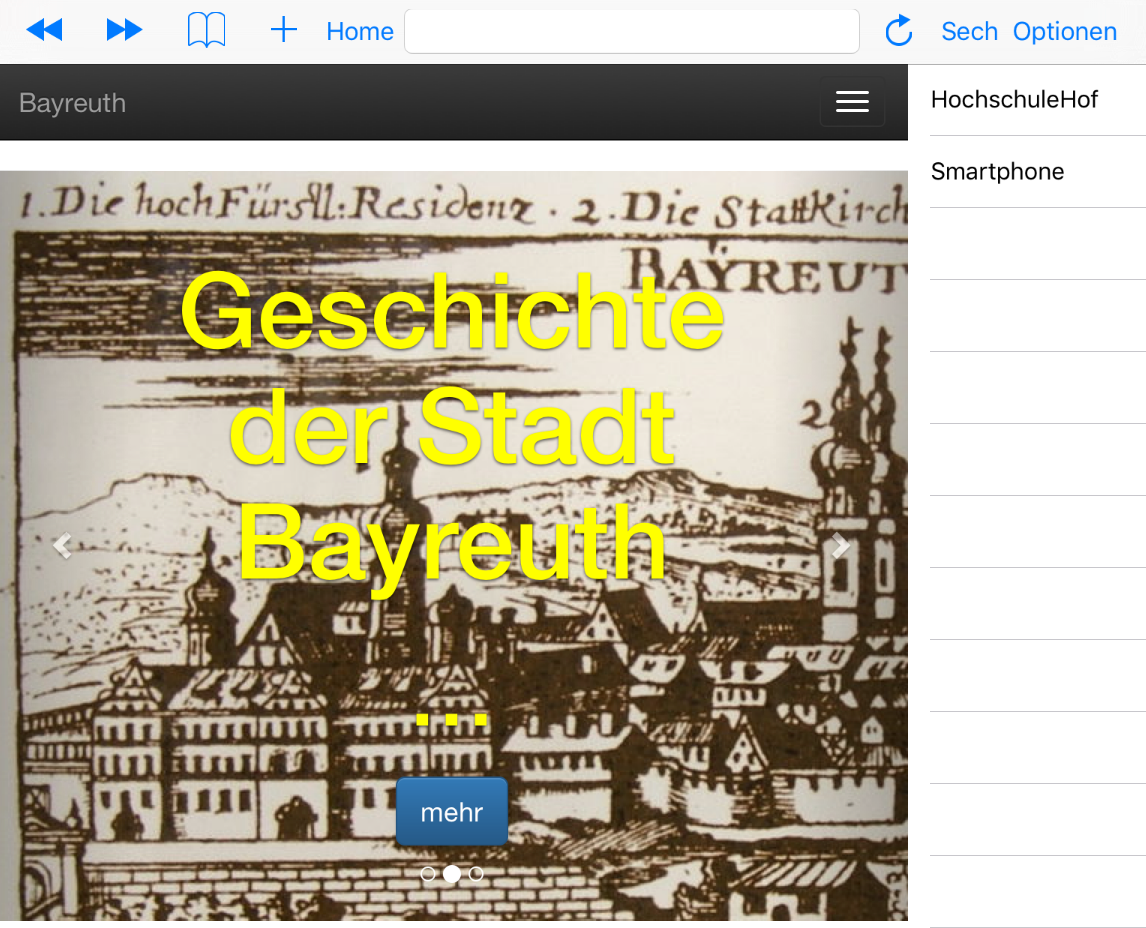
\includegraphics[width=12cm]{Pics/Browser_Hochformat}


